\chapter{Perancangan}
\label{chap:perancangan}
Pada bab ini akan dijelaskan perancangan program yang dibuat pada penelitian ini. Perancangan terdiri dari masukan program dan aktivitas sistem. 

\section{Masukan Program}
\label{sec:inputConfig} 
Program perekaman kehadiran daring otomatis membutuhkan 1 file sebagai masukan, yaitu \textit{file} .ini (\textit{file} konfigurasi). Pada \textit{file} .ini, nomor baris sebagai \textit{keys} dan \textit{string} berupa kata yang merupakan fungsi dari Selenium WebDriver dan elemen yang diambil untuk melakukan perekaman kehadiran daring otomatis sebagai \textit{values}. 

\subsection{Perancangan Masukan Program}
\label{sec:spek}
Pada subbab ini akan dijelaskan perancangan dari \textit{file} konfigurasi yang menjadi masukan untuk program. Gambar \ref{fig:spek} merupakan rancangan untuk \textit{file} konfigurasi.
\begin{figure}[H]
	\centering
	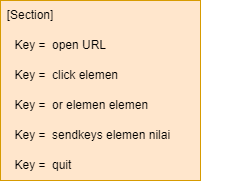
\includegraphics[scale=0.7]{Gambar/strukturConf.png}
	\caption{Gambar Rancangan Untuk Masukan Program} 
	\label{fig:spek}
\end{figure}
Penjelasan dari Gambar \ref{fig:spek} sebagai berikut:
\begin{itemize}
	\item \textit{File} konfigurasi memiliki \textit{section} dan nama \textit{section} dapat diubah sesuai keinginan. Nama \textit{section} ini yang akan dipanggil di dalam program, agar program dapat mengetahui seluruh isi \textit{key} dan \textit{value} dari \textit{file} konfigurasi tersebut.
	\item \textit{Key} akan berisi angka secara terurut dan dimulai dari angka satu hingga seterusnya. Diisi dengan angka secara terurut untuk memudahkan program dalam membaca langkap pertama hingga langkah terakhir.
	\item \textit{Value} terdiri dari kata kunci \textit{open}, \textit{click}, \textit{or}, \textit{sendkeys}, dan \textit{quit} yang berguna untuk program menjalankan perintah. \textit{Value} terdiri juga dari alamat web atau URL, elemen, dan nilai.
	\item Kata \textit{open} berpasangan dengan URL, karena kata \textit{open} merupakan kata kunci dari \textit{file} .ini bagi program untuk menjalankan fungsi \textit{get()} dari selenium, yaitu membuka situs web yang ingin dituju.
	\item Kata \textit{click} berpasangan dengan satu elemen, karena kata \textit{click} merupakan kata kunci dari \textit{file} .ini bagi program untuk menjalankan fungsi \textit{click} dari selenium, yaitu menekan suatu tombol secara otomatis sesuai dengan elemen yang telah diambil pada situs web yang telah dibuka.
	\item Kata \textit{sendkeys} berpasangan dengan satu elemen dan satu nilai, karena kata \textit{sendkeys} merupakan kata kunci dari \textit{file} .ini bagi program untuk menjalankan fungsi \textit{sendkeys()} dari selenium, yaitu mengetik atau memasukan suatu nilai dalam bentuk teks maupun angka secara otomatis pada suatu elemen yang telah diambil.
	\item Kata \textit{or} berpasangan dengan dua elemen, karena kata \textit{or} merupakan kata kunci dari \textit{file} .ini bagi program untuk menjalankan fungsi \textit{click()} dari selenium. Perbedaan dengan kata \textit{click} adalah bahwa kata \textit{or} ini diberi dua elemen dari web yang kemungkinan dapat terjadi dua-duanya atau salah satu saja. Lalu menekan tombol secara otomatis pada satu elemen yang telah diambil atau menekan tombol secara otomatis dua elemen yang telah diambil secara bertahap.  
	\item Kata \textit{quit} merupakan kata kunci dari \textit{file} .ini bagi program untuk menjalankan fungsi \textit{quit()} dari selenium, yaitu menutup browser.
\end{itemize}

\subsection{Konstruksi Masukan Program}
Konstruksi untuk masukan program dapat disusun setelah mengetahui rancangan dari masukan program yang sudah dibahas pada subbab \ref{sec:spek}. Konstruksi untuk masukan program dibuat dengan mengikuti langkah-langkah dari perekaman kehadiran daring secara manual. Hal ini dilakukan agar program dapat menjalankan perintah sesuai dengan langkah-langkah dari perekaman kehadiran daring secara manual. Pada subbab \ref{sec:alur} sudah dijelaskan alur untuk melakukan perekaman kehadiran daring mahasiswa secara manual dan tinggal diubah ke dalam file konfigurasi berdasarkan aturan dari rancangan dari masukan program, sehingga menghasil sebuah file konfigurasi esuai dengan alur perekaman kehadiran daring mahasiswa yang dapat dilihat pada Listing \ref{kode:4:conf}
\begin{lstlisting}[caption=Contoh \textit{file} .ini untuk Masukan Program Perekaman Kehadiran Daring Otomatis, label=kode:4:conf]
	[database_config]
	1 = open https://studentportal.unpar.ac.id
	2 = click #login-button
	3 = sendkeys #username 2017730035@student.unpar.ac.id 
	4 = click #next_login
	5 = sendkeys #password 12345
	6 = click #appPass>div.login__form>button
	7 = or a[href='https://studentportal.unpar.ac.id/jadwal'] .swal-button.swal-button--confirm.swal-button--danger
	8 = click a[onclick="absenPerkuliahan(this)"]
	9 = click .swal-button.swal-button--confirm.swal-button--danger9
	10 = quit
\end{lstlisting}
Berikut ini penjelasan dari isi pada file .ini yang merupakan masukan program perekaman kehadiran daring otomatis:
\begin{itemize}
	\item 1 = open https://studentportal.unpar.ac.id, merupakan langkah pertama untuk melakukan absensi, yaitu membuka situs web Portal Akademik Mahasiswa dengan kata kunci \textit{open} dan mengambil alamat situs web Portal Akademik Mahasiswa.
	\item 2 = click \#login-button, langkah kedua dengan kata kunci \textit{click} untuk menekan tombol \textit{``LOGIN''} yang memiliki elemen (\#login-button) berdasarkan \textit{CSS selector} pada tombol \textit{``LOGIN''}.
	\item 3 = sendkeys \#username 2017730035@student.unpar.ac.id, langkah ketiga dengan dengan kata kunci \textit{sendkeys} untuk memasukan sebuah nilai (2017730035@student.unpar.ac.id) pada elemen (\#username) yang merupakan tempat untuk memasukan \textit{email}.
	\item 4 = click \#next\_login, langkah keempat dengan kata kunci \textit{click} untuk menekan tombol \textit{``NEXT''} dan mengambil element (\#next\_login) pada tombol \textit{``NEXT''}.
	\item 5 = sendkeys \#password 12345, langkah kelima dengan kata kunci \textit{sendkeys} untuk memasukan sebuah nilai (12345) pada elemen (\#password) yang merupakan tempat untuk memasukan \textit{password}.
	\item 6 = click \#appPass>div.login\_\_form>button, langkah keenam dengan kata kunci \textit{click} untuk menekan tombol \textit{``LOGIN''} yang memiliki elemen (\#appPass>div.login\_\_form>button) agar dapat masuk ke dalam halaman utama situs Portal Akademik Mahasiswa. 
	\item 7 = or a[href='https://studentportal.unpar.ac.id/jadwal'] \\ .swal-button.swal-button--confirm.swal-button--danger, langkah ketujuh dengan kata kunci \textit{or} untuk membuat program melihat kondisi jika notifikasi peringatan muncul maka menekan tombol ``TUTUP'' dengan elemen (.swal-button.swal-button--confirm.swal-button--danger) lalu menekan tombol untuk masuk ke bagian halaman absensi dengan elemen (a[href='https://studentportal.unpar.ac.id/jadwal']), jika notifikasi peringatan tidak muncul maka langsung menekan tombol untuk masuk ke bagian halaman absensi dengan elemen \\ (a[href='https://studentportal.unpar.ac.id/jadwal']).
	\item 8 = click a[onclick="absenPerkuliahan(this)"], langkah kedelapan dengan kata kunci \textit{click} untuk menekan tombol absensi yang memiliki elemen (a[onclick="absenPerkuliahan(this)"]).
	\item 9 = click .swal-button.swal-button--confirm.swal-button--danger9, langkah kesembilan dengan kata kunci \textit{click} untuk menekan tombol \textit{``OK''} yang memiliki elemen (.swal-button.swal-button--confirm.swal-button--danger9) dari notifikasi yang menunjukan absensi telah berhasil.
	\item 10 = quit, langkah terakhir dengan kata kunci \textit{quit} untuk keluar dari browser.
\end{itemize}

\begin{figure}[H]
	\centering
	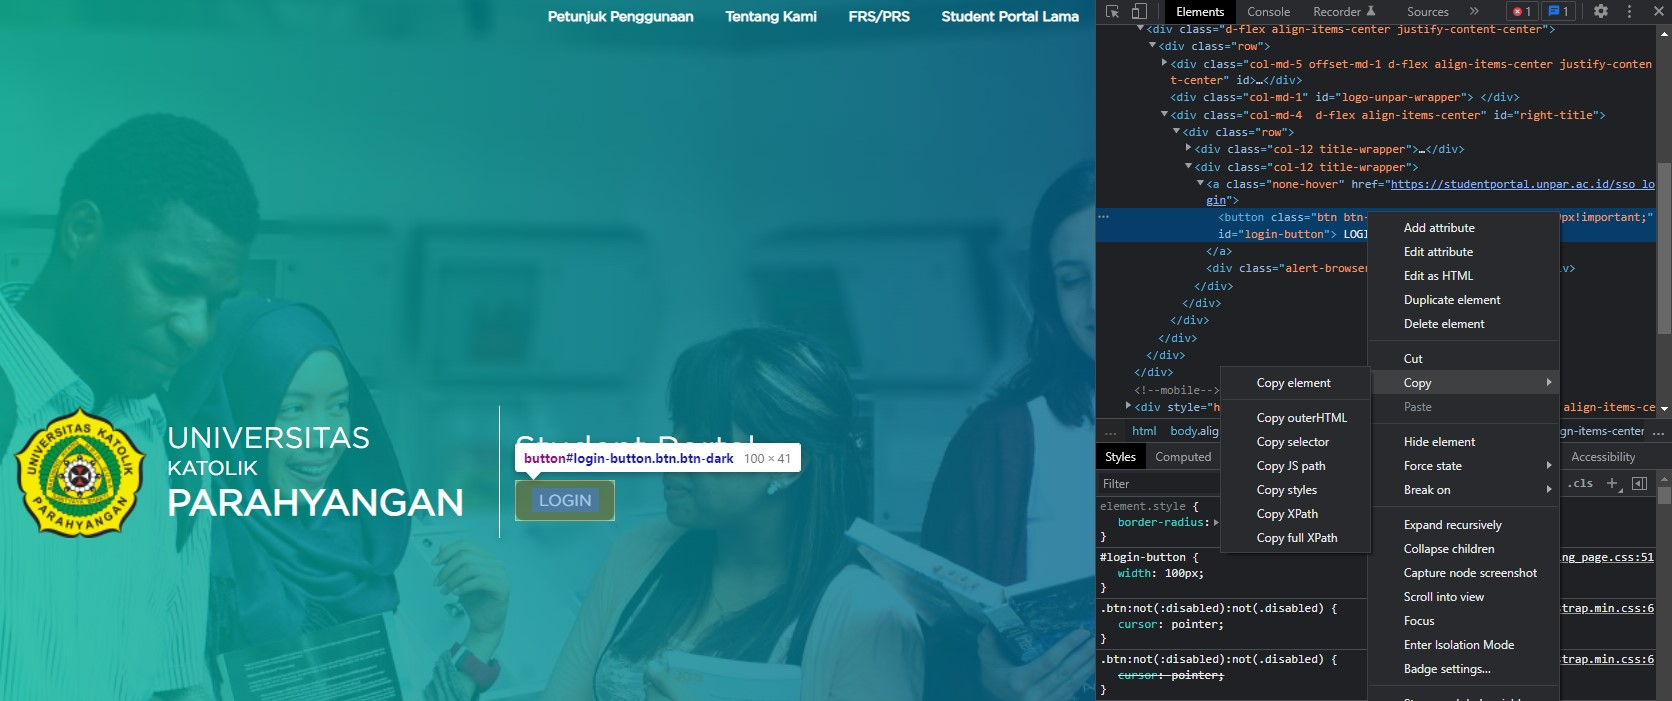
\includegraphics[scale=0.3]{Gambar/elemen.jpg}
	\caption{Tampilan Melakukan \textit{Inspect Element}} 
	\label{fig:inspect}
\end{figure}	
Elemen yang dipakai dalam \textit{file} .ini ini diambil dengan cara melakukan \textit{inspect element} pada web yang ingin dilakukan otomatisasi. Elemen yang dipilih berdasarkan \textit{CSS Selector} yang sudah dibahas pada subbab \ref{sec:terjemah}. Pada Gambar \ref{fig:inspect} adalah cara yang dilakukan untuk mendapat elemen yang ingin digunakan untuk otomatisasi. Untuk mendapatkan elemen tersebut, perlu melakukan klik kanan pada bagian elemen yang ingin diambil, lalu pilih ``inspect''. Setelah melakukan ``inspect'' maka akan muncul dokumen HTML yang dapat dilihat pada bagian kanan Gambar \ref{fig:inspect}, sehingga dapat melakukan pengambilan elemen yang diperlukan.

\section{Aktivitas Sistem}
\label{sec:diagramAktivitas}
Program perekaman absen daring otomatis adalah program yang digunakan untuk melakukan absensi secara otomatis bagi mahasiswa UNPAR. Program ini menggunakan Selenium WebDriver sebagai \textit{tools} yang berguna untuk melakukan otomatisasi pada browser web. Program ini juga membutuhkan masukan dari sebuah file konfigurasi untuk menjalankannya. Berikut ini adalah langkah-langkah yang harus dilakukan jika ingin menggunakan program ini:
\begin{enumerate}
	\item Pengguna melakukan \textit{install} python, karena program perekaman absen daring otomatis menggunakan bahasa pemrograman python.
	\item Pengguna melakukan \textit{install} selenium, karena untuk melakukan perekaman absen daring secara otomatis menggunakan selenium.
	\item Pengguna melakukan \textit{install} chrome driver sesuai versi dari browser Google Chrome, karena menggunakan browser Google Chrome untuk melakukan perekaman absen daring otomatis.
	\item Pengguna membuka file konfigurasi dan mengubah email serta password sesuai milik pengguna agar dapat digunakan sebagai masukan pada program untuk melakukan perekaman absen daring otomatis.
	\item Pengguna menyimpan hasil perubahan yang telah dilakukan pada file konfigurasi.
\end{enumerate}

Diagram Aktivitas untuk program perekaman kehadiran daring otomatis dapat dilihat pada Gambar \ref{fig:ActivityAplikasi}. Berikut ini adalah penjelasan pada diagram aktivitas:
\begin{enumerate}
	\item Pengguna menjalankan langsung programnya.
	\item Program akan membuka browser Google Chrome saat pertama kali program dijalankan.
	\item Program menerima masukan dari \textit{file} konfigurasi yang telah di-\textit{setup} oleh pengguna.
	\item Program akan menjalankan perintah sesuai masukan \textit{file} konfigurasi secara baris perbaris dimulai dari baris pertama.
	\item Setiap program selesai menjalankan satu baris perintah dari masukan \textit{file} konfigurasi maka program akan kembali melakukan cek baris berikutnya pada \textit{file} konfigurasi dan menjalankannya hingga baris terakhir.
	\item Jika masukan dari value \textit{file} konfigurasi terdapat kata \textit{open} maka program diberi perintah untuk membuka situs web yang dituju pada browser Google Chrome secara otomatis.
	\item Jika masukan dari value \textit{file} konfigurasi terdapat kata \textit{click} maka program diberi perintah untuk menekan suatu tombol yang diminta berdasarkan elemen yang telah diambil.
	\item Jika masukan dari value \textit{file} konfigurasi terdapat kata \textit{sendkeys} maka program diberi perintah untuk melakukan \textit{input} suatu nilai berupa angka atau kata ke dalam suatu elemen yang telah dipilih.
	\item Jika masukan dari value \textit{file} konfigurasi terdapat kata \textit{or} maka program akan menerima dua elemen secara langsung, jika elemen pertama telah ditemukan maka program langsung diberi perintah untuk menekan tombol berdasarkan elemen pertama, jika elemen kedua yang ditemukan terlebih dahulu maka program diberi perintah untuk menekan tombol berdasarkan elemen kedua terlebih dahulu lalu menekan tombol berdasarkan elemen pertama.
	\item Jika masukan dari value \textit{file} konfigurasi terdapat kata \textit{quit} maka program diberi perintah untuk menutup menutup browser dan program selesai dijalankan.

\end{enumerate}
\begin{figure}[H]
	\centering
	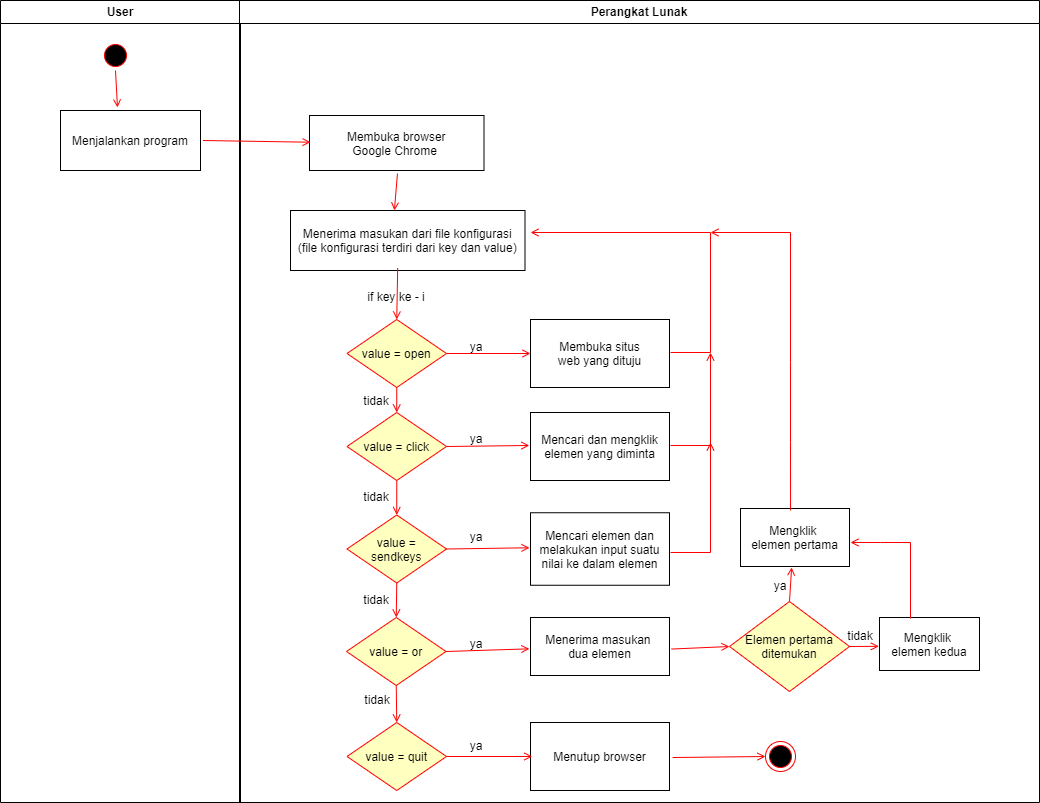
\includegraphics[scale=0.45]{Gambar/ActivityAplikasi.png}
	\caption{Diagram Aktivitas Program Absen Daring Otomatis} 
	\label{fig:ActivityAplikasi}
\end{figure}
\vspace{-0.3cm}
Pada diagram aktivitas program (Gambar \ref{fig:ActivityAplikasi}) hanya satu langkah saja yang dilakukan oleh pengguna untuk melakukan perekaman kehadiran daring, sedangkan pada diagram aktivitas absensi daring manual (Gambar \ref{fig:acPAM}) yang terletak pada subbab \ref{sec:alur} cukup banyak langkah yang perlu dilakukan untuk dapat melakukan perekaman kehadirang daring. Pengguna setidaknya perlu melakukan 10 langkah untuk dapat melakukan perekaman kehadiran daring secara manual. Program perekaman kehadiran daring otomatis ini mempersingkat langkah-langkah yang harus dilakukan pengguna untuk melakukan perekaman kehadiran daring dengan cukup menjalankan programnya.
\vspace{-0.4cm}
\section{Perancangan Algoritma} 
Perancangan algoritma ini memiliki \textit{input} berupa sebuah \textit{file} konfigurasi dan \textit{output} yang dihasilkan adalah program berhasil melakukan perekaman kehadiran daring. Algoritma ini akan melakukan perekaman kehadiran daring otomatis sesuai dari perintah masukan dari \textit{file} konfigurasi. 

\begin{algorithm} 
	\caption{Algoritma untuk Perekaman Kehadiran Daring  Otomatis}\label{euclid}
	\hspace*{\algorithmicindent} \textbf{Input: file\_konfigurasi} \\
	\hspace*{\algorithmicindent} \textbf{Output: Perekaman daring secara otomatis pada Google Chrome} 
	\begin{algorithmic}[1]
	% Input: 
	% Ouput: 
	\State $osPathEnvironment \gets getCurrentDirectory()$
	\State $driver \gets getChromeDriver()$ \Comment{Membuka browser}
	\State $parser \gets ConfigParser()$
	\State $parser.read(file\_konfigurasi)$
	\State $index \gets 1$
	\While{$TRUE$}
	\State $(command, parameters) \gets parser.get(file\_konfigurasi, str(index)).split()$
	\If {$command = "open"$}
	\State $driver.get(parameters[0])$  \Comment{Membuka situs yang dituju}
	\State $index \gets index + 1$
	\ElsIf {$command = "click"$}
	\State $elemen \gets findElementByCssSELECTOR(parameters[0])$
	\If {$elemenIsDisplayed()$ $AND$ $elemenIsEnabled()$}
	\State $elemen.click()$
	\Else 
	\State $driver.quit()$
	\State $print$ ($Absensi$ $Gagal$)
	\State $index \gets index + 1$
	\EndIf
	\ElsIf {$command = "sendkeys"$}
	\State $inpt \gets findElementByCssSELECTOR(parameters[0])$
	\State $inpt.send\_keys(parameters[1])$
	\State $index \gets index + 1$
	\ElsIf {$command = "or"$}
	\State $elemen1 \gets findElementByCssSELECTOR(parameters[0])$
	\State $elemen2 \gets findElementByCssSELECTOR(parameters[1])$
	\If {$elemenIsDisplayed()$ $AND$ $elemenIsEnabled()$}
	\State $elemen2.click()$
	\State $elemen1.click()$
	\Else
	\State $elemen1.click()$
	\State $index \gets index + 1$
	\EndIf
	\ElsIf {$command = "quit"$}
	\State $driver.quit() $  \Comment{Menutup browser}
	\State $print$ ($Absensi$ $Berhasil$)
	\EndIf
	\EndWhile
	\end{algorithmic}
\end{algorithm}